%%% ================================================
%%% OWASP Top 10 For LLM Applications Template
%%% Version: 0.0.1
%%% Date: 2023-11-28
%%% Template Authors:
%%%   - Jason Ross <algorythm@gmail.com>
%%% ================================================

%%% ================================================
%%% How to use this
%%% ================================================
%%% Update the variables below
%%% If you want to change text color on the front
%%% cover, the areas required are commented below.
%%% If you want to modify text and border colors
%%% for your chapter headers go into the file
%%% `structure.tex` and replace the name of the
%%% colour (set to ) with a new colour name
%%% (find and replace ctrl+f will do this for you).
%%% ================================================

%%% ================================================
%%%	VARIABLES
%%% ================================================

%%% Project Name
\def\projectName{LLM AI Cybersecurity \& Governance Checklist}
\def\projectSubName{From the OWASP Top 10 \\ for LLM Applications Team}
\def\docVersion{1.1}

%%% Project Type
\def\projectType{OWASP Project Document}

%%% Report Date (defaults to Today's date)
% \def\date{\today}
\def\date{April 11, 2024}


%%% ================================================
%%%	DOCUMENT CONFIGURATION
%%% ================================================

\documentclass[
        11pt,         % Default font size, select one of 10pt, 11pt or 12pt
        fleqn,        % Left align equations
        letterpaper,  % Paper size, use either 'a4paper' for A4 size or 'letterpaper' for US letter size
        % landscape,    % Uncomment for for a landscape layout (useful for wide tables or figures)
        oneside,      % Uncomment for oneside mode: this doesn't start new chapters and parts on odd pages (adding an empty page if required)
                      % this mode is more suitable if the book is to be read on a screen instead of printed
]{owasp-doc}


%%% ================================================
%%% DOCUMENT BEGINS HERE
%%% ================================================
% \tracingmacros=1 % turn on tracing
\begin{document}

\pagestyle{fancy}

%%%	COVER PAGE
% !TEX root = owasp-doc.tex

\pagestyle{empty}

%%% Background images
\AddToShipoutPicture*{\put(0,0){
\includegraphics{FrontCover.jpg}}}
\AddToShipoutPicture*{\put(0,0){
\includegraphics[width=8.5in, height=11in]{owasp_wasp1.png}}}

\vfill

\begingroup

%%% OWASP logo
\begin{figure}[t]

\includegraphics[width=0.6\textwidth,left]{owasp_logo.png}
\end{figure}

\begin{center}
    \par\normalfont\fontsize{42}{42}\sffamily\selectfont
    \vspace*{2.75cm}
    \textbf{\projectName}\par
\end{center}

\vspace*{10cm}
    \par\normalfont\fontsize{22}{22}\sffamily\selectfont
    \textbf{\color{white}Version: \docVersion}\par
    \par\normalfont\fontsize{14}{14}\sffamily\selectfont
    \textit{\color{white}\textbf{Published}:\date}\par

\endgroup

\clearpage

%%%	CHANGELOG & DISCLAIMER
% !TEX root = owasp-doc.tex
%%% ================================================
%%%	CHANGELOG & DISCLAIMER
%%% ================================================
\vfill
% changelog
% !TEX root = owasp-doc.tex
%%% Changelog
\begin{figure}[t!]
\fontsize{14}{14}
\owaspbf{Revision History}
\fontsize{11}{11}
  \begin{versionhistory}
  \vhEntry{0.1}{2023-11-01}{Sandy Dunn}{initial draft}
  \vhEntry{0.5}{2023-12-05}{Sandy Dunn, OWASP LLM Apps Team}{public draft}
\end{versionhistory}
\end{figure}
\vfill
% disclaimer
% !TEX root = owasp-doc.tex
%%% Disclaimer
\textit{The information provided in this document does not, and is not intended
to, constitute legal advice. All information is for general informational
purposes only.\\
\\
This document contains links to other third-party websites. Such links are only
for convenience and OWASP does not recommend or endorse the contents of the
third-party sites.
}
\vspace{2cm}
\owasplogobottomright
\clearpage

%%%	TABLE OF CONTENTS
% !TEX root = owasp-doc.tex

\headerimage
\tableofcontents

% if you want a list of tables included at the
% start of the document uncomment the next line
%\listoftables
\clearpage

%%% ALL OTHER CONTENT
% !TEX root = owasp-doc.tex

%%% ================================================
%%%	MAIN SECTIONS
%%% ================================================

% !TEX root = owasp-doc.tex

% ================================================
%	OVERVIEW
% ================================================

\headerimage
\chapter{Overview}
Every internet user and company should prepare for the upcoming wave of powerful generative artificial intelligence (GenAI) applications. GenAI has enormous promise for innovation, efficiency, and commercial success across a variety of industries. Still, like any powerful early stage technology, it brings its own set of obvious and unexpected challenges.

Artificial intelligence has advanced greatly over the last 50 years, inconspicuously supporting a variety of corporate processes until ChatGPT's public appearance drove the development and use of Large Language Models (LLMs) among both individuals and enterprises. Initially, these technologies were limited to academic study or the execution of certain, but vital, activities within corporations, visible only to a select few. However, recent advances in data availability, computer power, GenAI capabilities, and the release of tools such as Llama 2, ElevenLabs, and Midjourney have raised AI from a niche to general widespread acceptance. These improvements have not only made GenAI technologies more accessible, but they have also highlighted the critical need for enterprises to develop solid strategies for integrating and exploiting AI in their operations, representing a huge step forward in how we use technology.


\begin{itemize}
  \item \textbf{Artificial intelligence} (AI)  is a broad term that encompasses all fields of computer science that enable machines to accomplish tasks that would normally require human intelligence. Machine learning and generative AI are two subcategories of AI.
  \item \textbf{Machine learning} (ML) is a subset of AI that focuses on creating algorithms that can learn from data. Machine learning algorithms are trained on a set of data, and then they can use that data to make predictions or decisions about new data.
  \item \textbf{Generative AI} is a type of machine learning that focuses on creating new data. Often, GenAI relies on the use of large language models to perform the tasks needed to create the new data.
  \item A \textbf{large language model (LLM)} is a type of AI model that processes and generates human-like text. In the context of artificial intelligence a "model" refers to a system that is trained to make predictions based on input data. LLMs are specifically trained on large data sets of natural language and the name large language models.

\end{itemize}

Organizations are entering uncharted territory in securing and overseeing GenAI solutions. The rapid advancement of GenAI also opens doors for adversaries to enhance their attack strategies, introducing a dual challenge of defense and threat escalation.

\clearpage

Businesses use artificial intelligence in many areas, including HR for recruiting, email spam screening, SIEM for behavioral analytics, and managed detection and response applications. However, this document's primary focus is on Large Language Model applications and their function in creating generated content.

\section{Responsible and Trustworthy Artificial Intelligence}
As challenges and benefits of Artificial Intelligence emerge - and regulations and laws are passed - the principles and pillars of responsible and trustworthy AI usage are evolving from idealistic objects and concerns to established standards.
The \href{https://owasp-ai-exchange.web.app/}{OWASP AI Exchange Working Group} is monitoring these changes and addressing the broader and more challenging considerations for all aspects of artificial intelligence.

\begin{figure}[h]
  \centering
  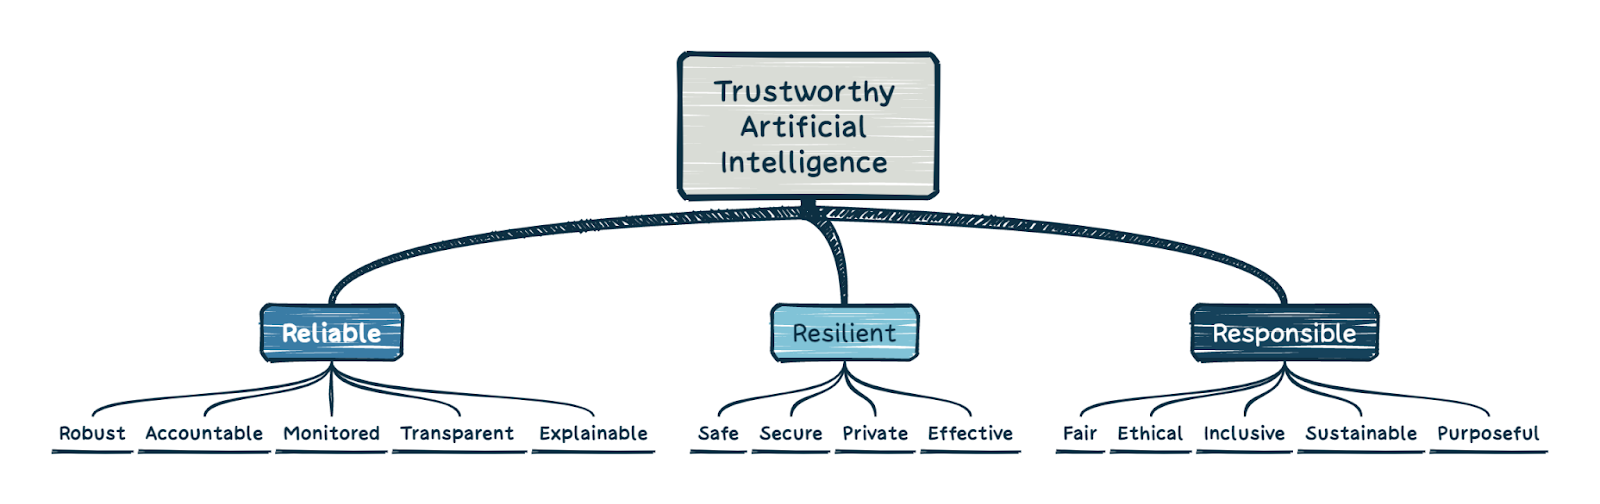
\includegraphics[width=\textwidth]{pillars_of_trustworthy_ai}
  \caption{Image depicting Pillars of Trustworthy Artificial Intelligence: created from Montreal Ethics Institute Example}
  \label{fig:pillars-of-trustworthy-ai}
\end{figure}

\clearpage

\section{Who is This For?}
The OWASP Top 10 for LLM Applications Cybersecurity and Governance Checklist is for leaders across executive, tech, cybersecurity, privacy, compliance, and legal areas, DevSecOps, MLSecOps, and Cybersecurity teams and defenders. It is intended for people who are striving to stay ahead in the fast-moving AI world, aiming not just to leverage AI for corporate success but also to protect against the risks of hasty or insecure AI implementations. These leaders and teams must create tactics to grab opportunities, combat challenges, and mitigate risks.

This checklist is intended to help these technology and business leaders quickly understand the risks and benefits of using LLM, allowing them to focus on developing a comprehensive list of critical areas and tasks needed to defend and protect the organization as they develop a Large Language Model strategy.

It is the hope of the OWASP Top 10 for the LLM Applications team that this list will help organizations improve their existing defensive techniques and develop techniques to address the new threats that come from using this exciting technology.

\section{Why a Checklist?}
Checklists used to formulate strategies improve accuracy, define objectives, preserve uniformity, and promote focused deliberate work, reducing oversights and missed details. Following a check list not only increases trust in a safe adoption journey, but also encourages future organizations innovations by providing a simple and effective strategy for continuous improvement.

\section{Not Comprehensive}
Although this document intends to support organizations in developing an initial LLM strategy in a rapidly changing technical, legal, and regulatory environment, it is not exhaustive and does not cover every use case or obligation. While using this document is Organizations should extend assessments and practices beyond the scope of the provided checklist as required for their use case or jurisdiction.

\section{Large Language Model Challenges}
Large Language models face several serious and unique issues. One of the most important is that while working with LLMs, the control and data planes cannot be strictly isolated or separable. Another significant challenge is that LLMs are nondeterministic by design, yielding a different outcome when prompted or requested. LLMs employ semantic search rather than keyword search. The key distinction between the two is that the model's algorithm prioritizes the terms in its response. This is a significant departure from how consumers have previously used technology, and it has an impact on the consistency and reliability of the findings. Hallucinations, emerging from the gaps and training flaws in the data the model is trained on, are the result of this method.

There are methods to improve reliability and reduce the attack surface for jailbreaking, model tricking, and hallucinations, but there is a trade-off between restrictions and utility in both cost and functionality.

LLM use and LLM applications increase an organization's attack surface. Some risks associated with LLMs are unique, but many are familiar issues, such as the known software bill of materials (SBoM), supply chain, data loss protection (DLP), and authorized access. There are also increased risks not directly related to GenAI, but GenAI increases the efficiency, capability, and effectiveness of attackers who attack and threaten organizations.

Adversaries are increasingly harnessing LLM and Generative AI tools to refine and expedite traditional methods of attacking organizations, individuals, and government systems. LLM facilitates their ability to enhance techniques allowing them to effortlessly craft new malware, potentially embedded with novel zero-day vulnerabilities or designed to evade detection. They can also generate sophisticated, unique, or tailored phishing schemes. The creation of convincing deep fakes, whether video or audio, further promotes their social engineering ploys. Additionally, these tools enable them to execute intrusions and develop innovative hacking capabilities. In the future, more “tailored” and compound use of AI technology by criminal actors will demand specific responses and dedicated solutions for an organization's appropriate defense and resilience capabilities.

Organizations also face the threat of NOT utilizing the capabilities of LLMs such as a competitive disadvantage, market perception by customers and partners of being outdated, inability to scale personalized communications, innovation stagnation, operational inefficiencies, the higher risk of human error in processes, and inefficient allocation of human resources.


Understanding the different kinds of threats and integrating them with the business strategy will help weigh both the pros and cons of using Large Language Models (LLMs) against not using them, making sure they accelerate rather than hinder the business's meeting business objectives.

\section{LLM Threat Categories}
\begin{figure}[h]
  \centering
  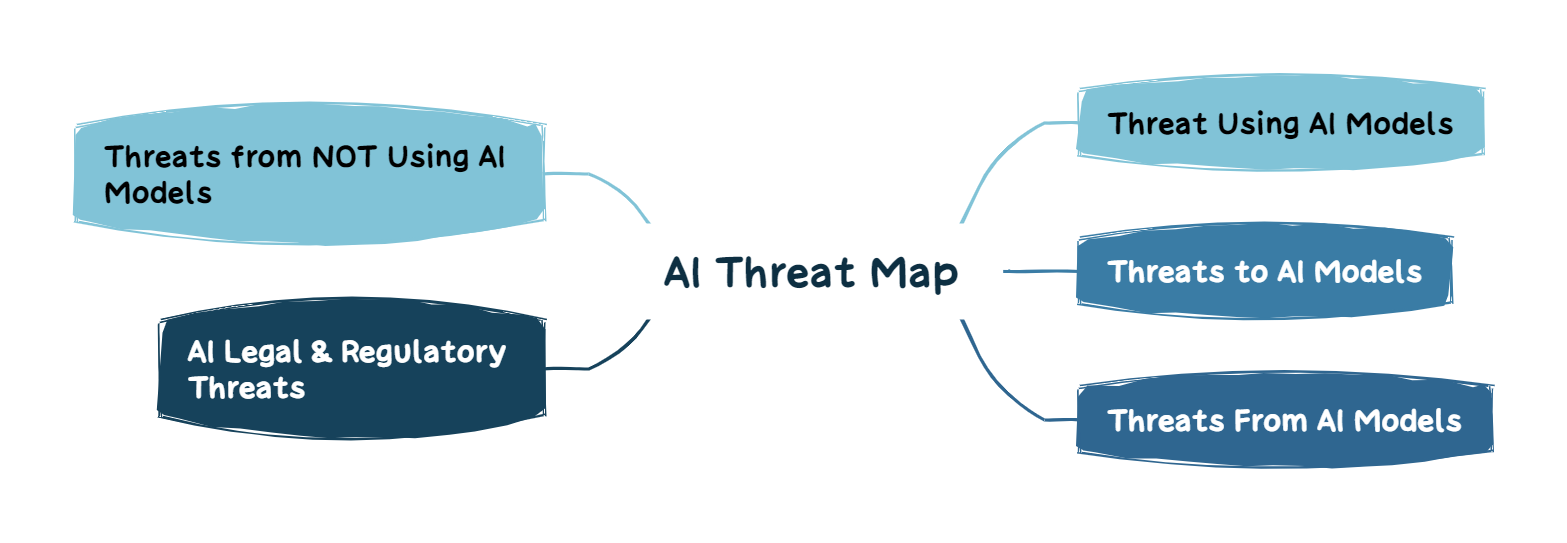
\includegraphics[width=\textwidth]{types_of_ai_threats}
  \caption{Image depicting the types of AI threats: credit sdunn}
  \label{fig:types-of-ai-threats}
\end{figure}

\clearpage

\section{Artificial Intelligence Security and Privacy Training}
Employees throughout organizations benefit from training to understand artificial intelligence, generative artificial intelligence, and the future potential consequences of building, buying, or utilizing LLMs. Training for permissible use and security awareness should target all employees as well as be more specialized for certain positions such as human resources, legal, developers, data teams, and security teams.

Fair use policies and healthy interaction are key aspects that, if incorporated from the very start, will be a cornerstone to the success of future AI cybersecurity awareness campaigns. This will necessarily provide user's with knowledge of the basic rules for interaction as well as the ability to separate good behavior from bad or unethical behavior.


\section{Incorporate LLM Security and governance with Existing, Established Practices and Controls}
While AI and generated AI add a new dimension to cybersecurity, resilience, privacy, and meeting legal and regulatory requirements, the best practices that have been around for a long time are still the best way to identify issues, find vulnerabilities, fix them, and mitigate potential security issues.

\begin{itemize}
  \item Confirm the management of artificial intelligence systems is integrated with existing organizational practices.
  \item Confirm AIML systems follow existing privacy, governance, and security practices, with AI specific privacy, governance, and security practices implemented when required.
\end{itemize}

\section{Fundamental Security Principles}
LLM capabilities introduce a different type of attack and attack surface. LLMs are vulnerable to complex business logic bugs, such as prompt injection, insecure plugin design, and remote code execution. Existing best practices are the best way to solve these issues. An internal product security team that understands secure software review, architecture, data governance, and third-party assessments The cybersecurity team should also check how strong the current controls are to find problems that could be made worse by LLM, such as voice cloning, impersonation, or bypassing captchas.

Given recent advancements in machine learning, NLP (Natural Language Processing), NLU (Natural Language Understanding), Deep Learning, and more recently, LLMs (Large Language Models) and Generative AI, it is recommended to include professionals proficient in these areas alongside cybersecurity and devops teams. Their expertise will not only aid in adopting these technologies but also in developing innovative analyses and responses to emerging challenges.


\clearpage

\section{Risk}
Reference to risk uses the ISO 31000 definition: Risk = "effect of uncertainty on objectives." LLM risks included in the checklist includes a targeted list of LLM risks that address adversarial, safety, legal, regulatory, reputation, financial, and competitive risks.

\section{Vulnerability and Mitigation Taxonomy}
Current systems for classifying vulnerabilities and sharing threat information, like OVAL, STIX, CVE, and CWE, are still developing the ability to monitor and alert defenders about vulnerabilities and threats specific to Large Language Models (LLMs) and Predictive Models. It is expected that organizations will lean on these established and recognized standards, such as CVE for vulnerability classification and STIX for the exchange of cyber threat intelligence (CTI), when vulnerabilities or threats to AI/ML systems and their supply chains are identified.

% !TEX root = owasp-doc.tex
% ================================================
%	LLM Challenges
% ================================================
\headerimage
\chapter{Large Language Model Challenges}
Large Language models face a number of serious and unique issues. One of the
most important is that while working with LLMs, the control and data planes
cannot be strictly isolated or separable. Another significant challenge is
that LLMs are nondeterministic by design, yielding a different outcome when
prompted or requested. It is not always a challenge, but LLMs employ semantic
search rather than keyword search. The key distinction between the two is that
the model's algorithm prioritizes the terms in its response. This is a
significant departure from how consumers have traditionally used technology,
and it has an impact on the consistency and reliability of the findings.
Hallucinations, emerging from the gaps and training flaws in the data the model
is trained on, are the result of this method.

There are methods to improve reliability and reduce the attack surface for
jailbreaking, model tricking, and hallucinations, but there is a trade-off
between restrictions and utility in both cost and functionality.

LLM use and applications increase an organization's attack surface. Some risks
associated with LLMs are unique, but many are familiar issues, such as the
known software bill of materials (SBOM), supply chain, data loss protection
(DLP), and authorized access. There are also increased risks not directly
related to GenAI, but GenAI increases the efficiency, capability, and
effectiveness of attacks.

Adversaries are increasingly harnessing LLM and Generative AI tools to refine
and expedite traditional methods. These enhanced techniques allow them to
effortlessly craft new malware, potentially embedded with novel zero-day
vulnerabilities or designed to evade detection. They can also generate
sophisticated, unique, or tailored phishing schemes. The creation of convincing
deep fakes, whether video or audio, further facilitates their social
engineering ploys. Additionally, these tools enable them to execute intrusions
and develop innovative hacking utilities. It is very likely that in the future,
more “tailored” and compound use of AI technology by criminal actors will demand
specific responses and dedicated solutions for appropriate defense schemas.

\clearpage
\section{LLM Threat Categories}
\begin{figure}[h]
  \centering
  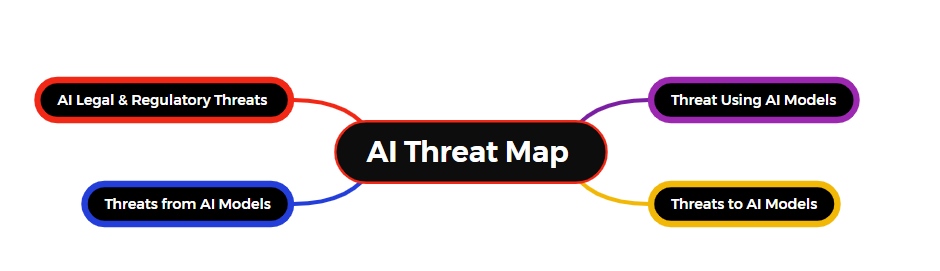
\includegraphics[width=\textwidth]{ai_threat_map}
  \caption{Image of types of AI threats}
  \label{fig:ai-threat-map}
\end{figure}

\section{Artificial Intelligence Security and Privacy Training}
Employees throughout organizations benefit from training to understand
artificial intelligence, generative artificial intelligence, and the future
potential consequences of building, buying, or utilizing LLMs. Training for
permissible use and security awareness should target all employees as well as
be more specialized for certain positions such as human resources, legal,
developers, data teams, and security teams.

Fair use policies and healthy interaction are key aspects that, if incorporated
from the very start, will be a cornerstone to the success of future AI
cybersecurity awareness campaigns. This will necessarily imply the user's
knowledge of the basic rules for interaction as well as the ability to separate
good behavior from bad or unethical behavior.

\section{Incorporate LLM Security and governance with Existing, Established Practices and Controls}
While AI and generated AI add a new dimension to cybersecurity, resilience,
privacy, and meeting legal and regulatory requirements, the best practices that
have been around for a long time are still the best way to find risks, test
them, fix them, and lower them.

\begin{itemize}
  \item The management of artificial intelligence systems is integrated with
  existing organizational practices.
  \item Apply existing privacy, governance, and security practices.
\end{itemize}

\clearpage
\section{Fundamental Security Principles}
LLM capabilities introduce a different type of attack and attack surface. LLMs
are vulnerable to complex business logic bugs, such as prompt injection,
insecure plugin design, and remote code execution. Existing best practices are
the best way to solve these issues. An internal product security team that
understands secure software review, architecture, data governance, and
third-party assessments The cybersecurity team should also check how strong
the current controls are to find problems that could be made worse by LLM,
like voice cloning, impersonation, or getting around captchas.

Accounting for the specific skills and competences developed in the last few
years around machine learning, NLP and NLU, deep Learning and lately, LLMs and
GenAI, it is advised to have skilled professionals with practice, knowledge, or
experience in these fields to side with security teams in adopting, at best,
and even shaping new potential analyses and responses to those issues.

\section{Risk}
Reference to risk uses the ISO 31000 definition: Risk = "effect of uncertainty on objectives."
LLM risks included in the checklist include a targeted list of LLM risks that
address adversarial, safety, legal, regulatory, reputation, financial, and competitive risks.

\section{Vulnerability and Mitigation Taxonomy}
Established methods of vulnerability classification and threat sharing are in
early development, such as Oval, STIX, threat sharing, and vulnerability
classification. The checklist anticipates calibrating with existing,
established, and accepted standards, such as CVE classification.
% !TEX root = owasp-doc.tex

% ================================================
%	LLM Strategy
% ================================================

\headerimage
\chapter{Determining LLM Strategy}
The rapid expansion of Large Language Model (LLM) applications has heightened
the attention and examination of all AI/ML systems used in business operations,
encompassing both Generative AI and long-established Predictive AI/ML systems.
This increased focus exposes potential risks, such as attackers targeting
systems that were previously overlooked and governance or legal challenges that
may have been disregarded in terms of legal, privacy, liability, or warranty
issues. For any organization leveraging AI/ML systems in its operations, it's
critical to assess and establish comprehensive policies, governance, security
protocols, privacy measures, and accountability standards to ensure these
technologies align with business processes securely and ethically.

Attackers, or adversaries, provide the most immediate and harmful threat to
enterprises, people, and government agencies. Their goals, which range from
financial gain to espionage, push them to steal critical information, disrupt
operations, and damage confidence. Furthermore, their ability to harness new
technologies such as AI and machine learning increases the speed and
sophistication of attacks, making it difficult for defenses to stay ahead of
attacks.

The most pressing non-adversary LLM threat for many organizations stem from
"Shadow AI": employees using unapproved online AI tools, unsafe browser
plugins, and third-party applications that introduce LLM features via updates
or upgrades, circumventing standard software approval processes.

\begin{figure}[h]
  \centering
  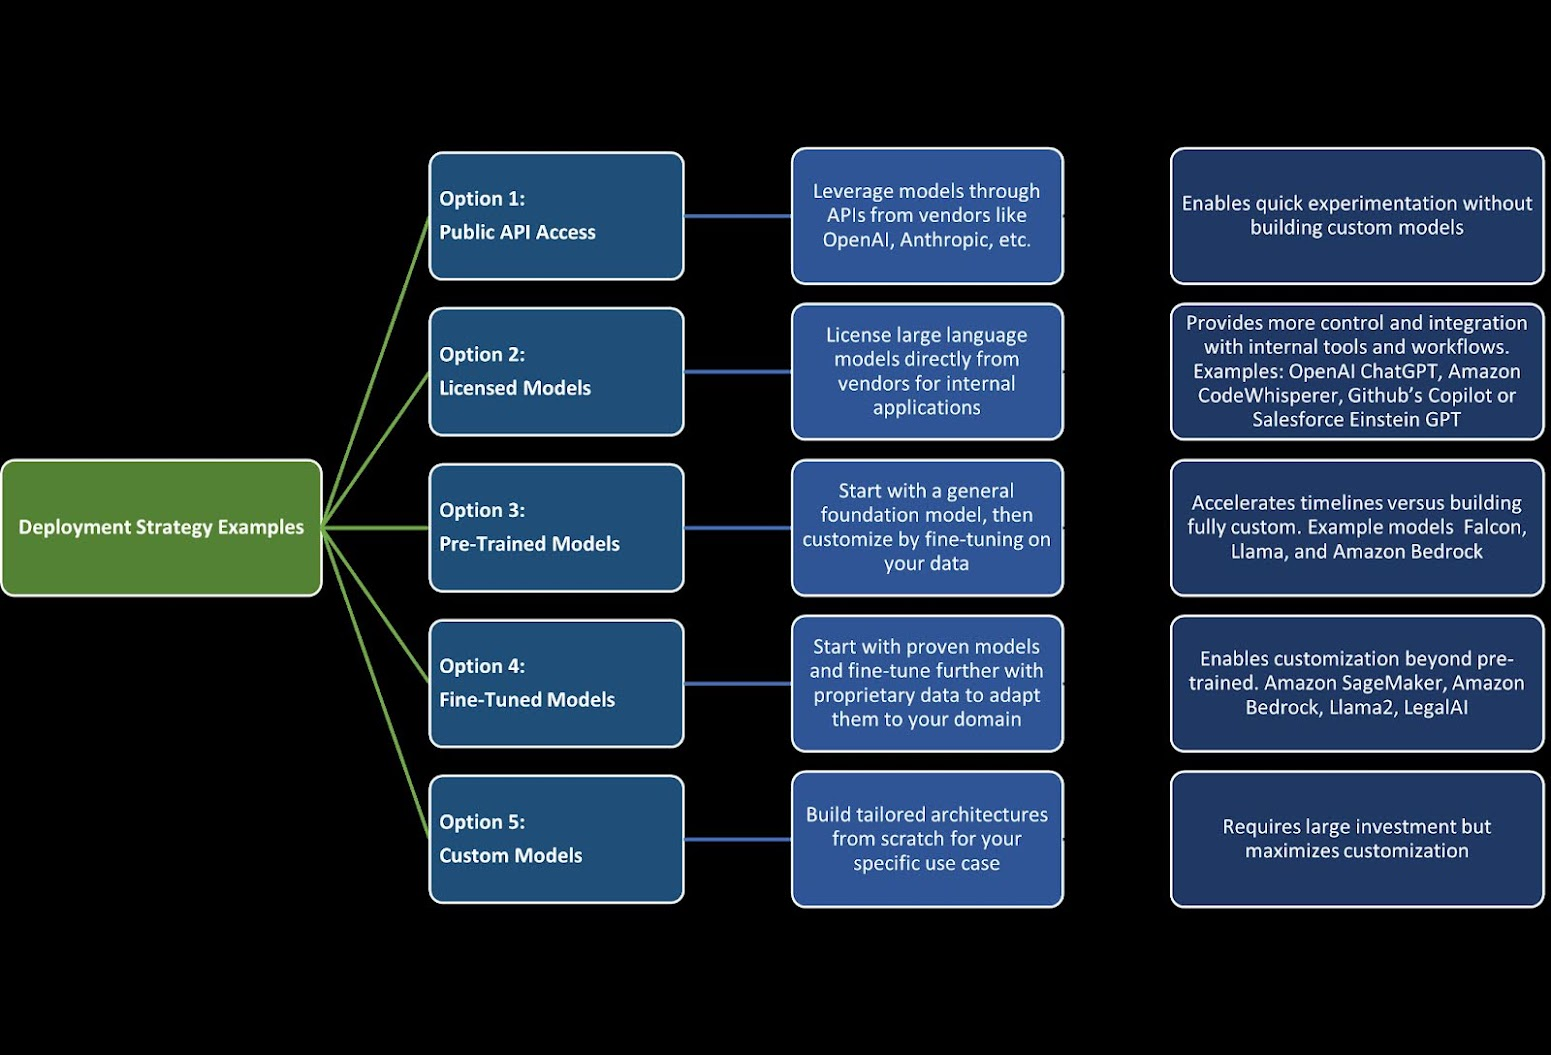
\includegraphics[width=\textwidth]{ai_deployment_strategy}
  \caption{Image of options for deployment strategy}
  \label{fig:llm-deployment-strategy}
\end{figure}

\clearpage

\section{Deployment Strategy}
The scopes range from leveraging public consumer applications to training
proprietary models on private data. Factors like use case sensitivity,
capabilities needed, and resources available help determine the right balance
of convenience vs. control. However, understanding these five model types
provides a framework for evaluating options.

\begin{figure}[h]
  \centering
  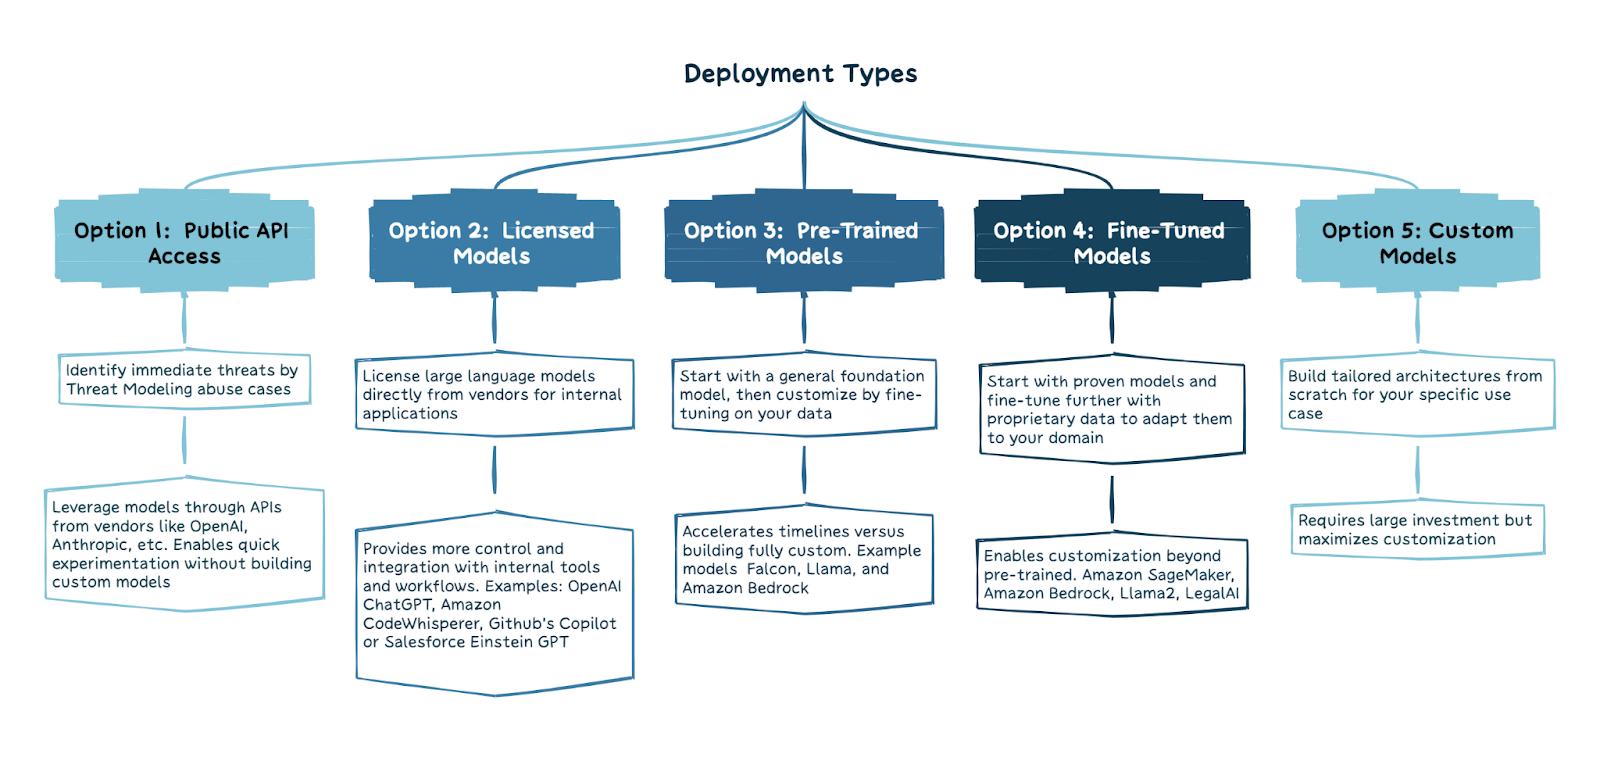
\includegraphics[width=\textwidth]{ai_deployment_types}
  \caption{Image of options for deployment types}
  \label{fig:llm-deployment-types}
\end{figure}

% !TEX root = owasp-doc.tex

% ================================================
%	LLM Strategy
% ================================================

\headerimage
\chapter{Check List}

\section{Adversarial Risk}
Adversarial Risk includes competitors and attackers.

\begin{minipage}{\linewidth}
\begin{checklist}
  \item Scrutinize how competitors are investing in artificial intelligence. Although there are risks in AI adoption, there are also business benefits that may impact future market positions.
  \item Threat Model: how attackers may accelerate exploit attacks against the organization, employees, executives, or users.
  \item Threat models potential attacks on customers or clients through spoofing and generative AI.
  \item Investigate the impact of current controls, such as password resets, which use voice recognition.
  \item Update the Incident Response Plan and playbooks for LLM incidents.
\end{checklist}
\end{minipage}

\section{AI Asset Inventory}
An AI asset inventory should apply to both internally developed and external or
third-party solutions.

\begin{minipage}{\linewidth}
\begin{checklist}
  \item Catalog existing AI services, tools, and owners. Designate a tag in asset management for specific inventory.
  \item Include AI components in the Software Bill of Material (SBOM), a comprehensive list of all the software components, dependencies, and metadata associated with applications.
  \item Catalog AI data sources and the sensitivity of the data (protected, confidential, public)
  \item Establish if pen testing or red teaming of deployed AI solutions is required to determine the current attack surface risk.
  \item Create an AI solution onboarding process.
  \item Ensure skilled IT admin staff is available either internally or externally, in accordance to the SBoM
\end{checklist}
\end{minipage}

\section{AI Security and Privacy Training}
\begin{minipage}{\linewidth}
\begin{checklist}
  \item Train all users on ethics, responsibility, and legal issues such as warranty, license, and copyright.
  \item Update security awareness training to include GenAI related threats. Voice cloning and image cloning, as well as in anticipation of increased spear phishing attacks
  \item Any adopted GenAI solutions should include training for both DevOps and cybersecurity for the deployment pipeline to ensure AI safety and security assurances.
\end{checklist}
\end{minipage}

\section{Establish Business Cases}
Solid business cases are essential to determining the business value of any
proposed AI solution,balancing risk and benefits, and evaluating and testing
return on investment. There are an enormous number of potential use cases; a
few examples are provided.

\begin{minipage}{\linewidth}
\begin{checklist}
  \item Enhance customer experience
  \item Better operational efficiency
  \item Better knowledge management
  \item Enhanced innovation
  \item Market Research and Competitor Analysis
  \item Document creation, translation, summarization, and analysis
\end{checklist}
\end{minipage}

\section{Governance}
Corporate governance in LLM is needed to provide organizations with transparency
and accountability. Identifying AI platform or process owners who are
potentially familiar with the technology or the selected use cases for the
business is not only advised but also necessary to ensure adequate reaction
speed that prevents collateral damages to well established enterprise digital
processes.

\begin{minipage}{\linewidth}
\begin{checklist}
  \item Establish the organization\'s AI RACI chart (who is responsible, who is accountable, who should be consulted, and who should be informed)
  \item Document and assign AI risk, risk assessments, and governance responsibility within the organization.
  \item Establish data management policies, including technical enforcement, regarding data classification and usage limitations. Models should only leverage data classified for the minimum access level of any user of the system. For example, update the data protection policy to emphasize not to input protected or confidential data into nonbusiness-managed tools.
  \item Create an AI Policy supported by established policy (e.g., standard of good conduct, data protection, software use)
  \item Publish an acceptable use matrix for various generative AI tools for employees to use.
  \item Document the sources and management of any data that the organization uses from the generative LLM models.
\end{checklist}
\end{minipage}

\section{Legal}
Many of the legal implications of AI are undefined and potentially very costly.
An IT, security, and legal partnership is critical to identifying gaps and
addressing obscure decisions.

\begin{minipage}{\linewidth}
\begin{checklist}
  \item Confirm product warranties are clear in the product development stream to assign who is responsible for product warranties with AI.
  \item Review and update existing terms and conditions for any GenAI considerations.
  \item Review AI EULA agreements. End-user license agreements for GenAI platforms are very different in how they handle user prompts, output rights and ownership, data privacy, compliance and liability, privacy, and limits on how output can be used.
  \item Review existing AI-assisted tools used for code development. A chatbot\'s ability to write code can threaten a company\'s ownership rights to its own product if a chatbot is used to generate code for the product. For example, it could call into question the status and protection of the generated content and who holds the right to use the generated content.
  \item Review any risks to intellectual property. Intellectual property generated by a chatbot could be in jeopardy if improperly obtained data was used during the generative process, which is subject to copyright, trademark, or patent protection. If AI products use infringing material, it creates a risk for the outputs of the AI, which may result in intellectual property infringement.
  \item Review any contracts with indemnification provisions. Indemnification clauses try to put the responsibility for an event that leads to liability on the person who was more at fault for it or who had the best chance of stopping it. Establish guardrails to determine whether the provider of the AI or its user caused the event, giving rise to liability.
  \item Review liability for potential injury and property damage caused by AI systems.
  \item Review insurance coverage. Traditional (D\&O) liability and commercial general liability insurance policies are likely insufficient to fully protect AI use.
  \item Identify any copyright issues. Human authorship is required for copyright. An organization may also be liable for plagiarism, propagation of bias, or intellectual property infringement if LLM tools are misused.
  \item Ensure agreements are in place for contractors and appropriate use of AI for any development or provided services.
  \item Restrict or prohibit the use of generative AI tools for employees or contractors where enforceable rights may be an issue or where there are IP infringement concerns.
  \item Assess and AI solutions used for employee management or hiring could result in disparate treatment claims or disparate impact claims.
  \item Make sure the AI solutions do not collect or share sensitive information without proper consent or authorization.
\end{checklist}
\end{minipage}

\section{Regulatory}
The EU AI Act is anticipated to be the first comprehensive AI law but will
apply in 2025 at the earliest. The EU\'s General Data Protection Regulation
(GDPR) does not specifically address AI but includes rules for data collection,
data security, fairness and transparency, accuracy and reliability, and
accountability, which can impact GenAI use. In the United States, AI regulation
is included within broader consumer privacy laws. Ten US states have passed
laws or have laws that will go into effect by the end of 2023.

Federal organizations such as the US Equal Employment Opportunity Commission
(EEOC), the Consumer Financial Protection Bureau (CFPB), the Federal Trade
Commission (FTC), and the US Department of Justice\'s Civil Rights Division
(DOJ) are closely monitoring hiring fairness.

\begin{minipage}{\linewidth}
\begin{checklist}
  \item Determine State specific compliance requirements.
  \item Determine compliance requirements for restricting electronic monitoring of employees and employment-related automated decision systems (Vermont)
  \item Determine compliance requirements for consent for facial recognition and the AI video analysis required (Illinois, Maryland)
  \item Review any AI tools in use or being considered for employee hiring or management.
  \item Confirm the vendor\'s compliance with applicable AI laws and best practices.
  \item Ask and document any products using AI during the hiring process. Ask how the model was trained, how it is monitored, and track any corrections made to avoid discrimination and bias.
  \item Ask and document what accommodation options are included.
  \item Ask and document whether the vendor collects confidential data.
  \item Ask how the vendor or tool stores and deletes data and regulates the use of facial recognition and video analysis tools during pre-employment.
  \item Review other organization-specific regulatory requirements with AI that may raise compliance issues. The Employee Retirement Income Security Act of 1974, for instance, has fiduciary duty requirements for retirement plans that a chatbot might not be able to meet.
\end{checklist}
\end{minipage}

\section{Using or Implementing Large Language Model Solutions}

\begin{minipage}{\linewidth}
\begin{checklist}
  \item Threat Model: LLM components and architecture trust boundaries.
  \item Data Security: Verify how data is classified and protected based on sensitivity, including personal and proprietary business data. (How are user permissions managed, and what safeguards are in place?)
  \item Access Control: Implement least privilege access controls and implement defense-in-depth measures
  \item Training Pipeline Security: Require rigorous control around training data governance, pipelines, models, and algorithms.
  \item Input and Output Security: Evaluate input validation methods, as well as how outputs are filtered, sanitized, and approved.
  \item Monitoring and Response: Map workflows, monitoring, and responses to understand automation, logging, and auditing. Confirm audit records are secure.
  \item Include application testing, source code review, vulnerability assessments, and red teaming in the production release process.
  \item Consider vulnerabilities in the LLM model solutions (Rezilion OSFF Scorecard).
  \item Look into the effects of threats and attacks on LLM solutions, such as prompt injection, the release of sensitive information, and process manipulation.
  \item Investigate the impact of attacks and threats to LLM models, including model poisoning, improper data handling, supply chain attacks, and model theft.
  \item Supply Chain Security: Request third-party audits, penetration testing, and code reviews for third-party providers. (both initially and on an ongoing basis)
  \item Infrastructure Security: How often does the vendor perform resilience testing? What are their SLAs in terms of availability, scalability, and performance?
  \item Update incident response playbooks and include an LLM incident in tabletop exercises.
  \item Identify or expand metrics to benchmark generative cybersecurity AI against other approaches to measure expected productivity improvements.
\end{checklist}
\end{minipage}
% !TEX root = owasp-doc.tex

% ================================================
%	Resources
% ================================================

\headerimage
\chapter{Resources}

\section{OWASP Top 10 for Large Language Model Applications}

\begin{figure}[ht]
  \centering
  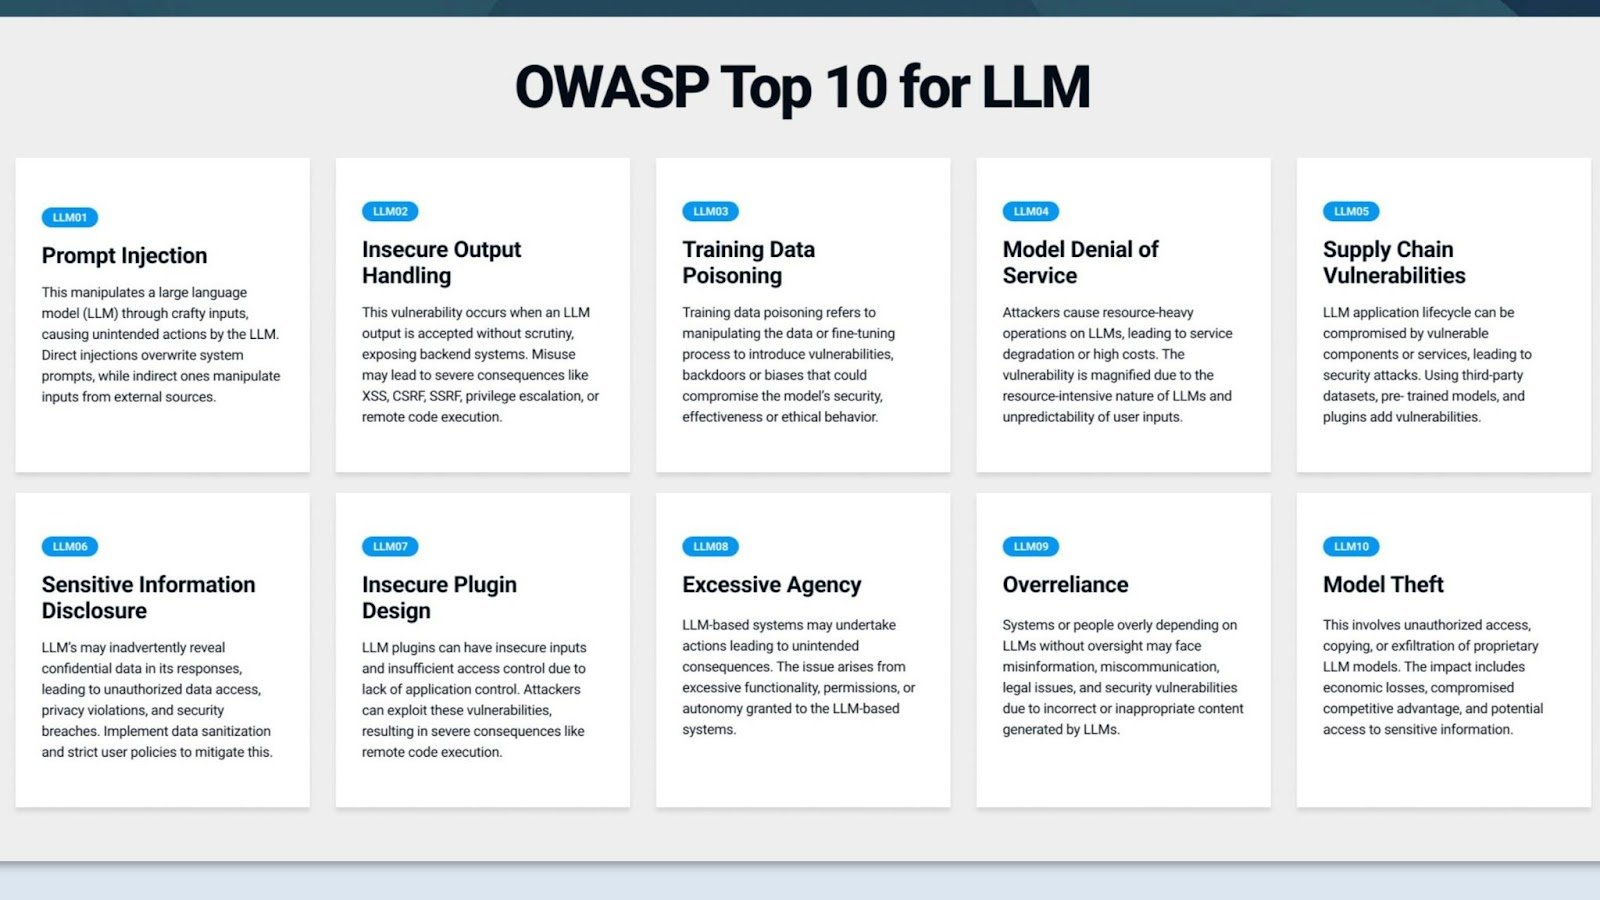
\includegraphics[width=0.8\textwidth]{owasp_top_10_llm_highlevel}
  \caption{Image of OWASP Top 10 for Large Language Model Applications}
  \label{fig:owasp-top-10-llm-highlevel}
\end{figure}

\clearpage
\section{OWASP Top 10 for Large Language Model Applications Visualized}

\begin{figure}[ht]
  \centering
  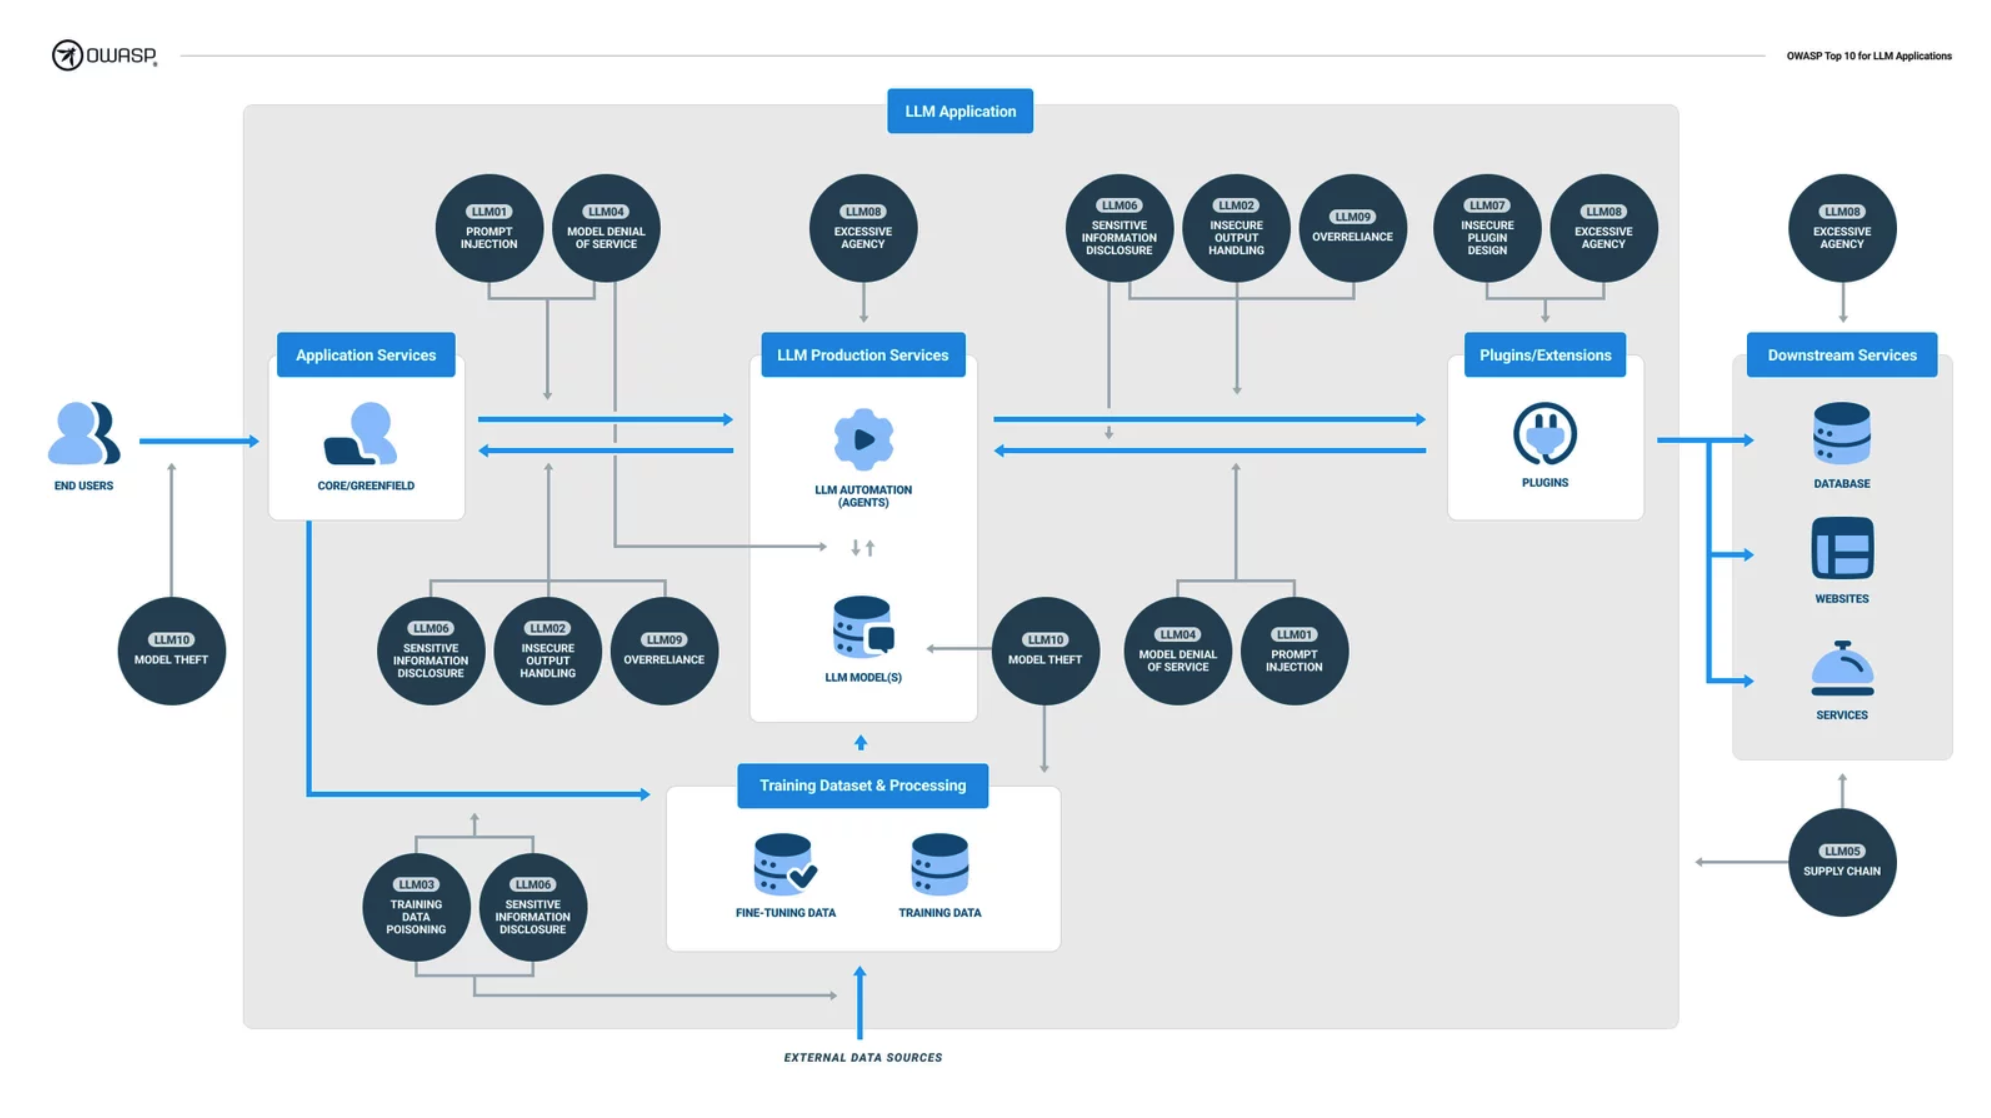
\includegraphics[width=0.8\textwidth]{owasp_top_10_llm_app_arch}
  \caption{Image of OWASP Top 10 for Large Language Model Applications Visualized}
  \label{fig:owasp-top-10-llm-visualized}
\end{figure}

% !TEX root = owasp-doc.tex
% \clearpage %%% Since this is the first section in the resources chapter, we don't clear the page

\textbf{OWASP Top 10 for Large Language Model Applications}
\begin{figure}[ht]
  \centering
  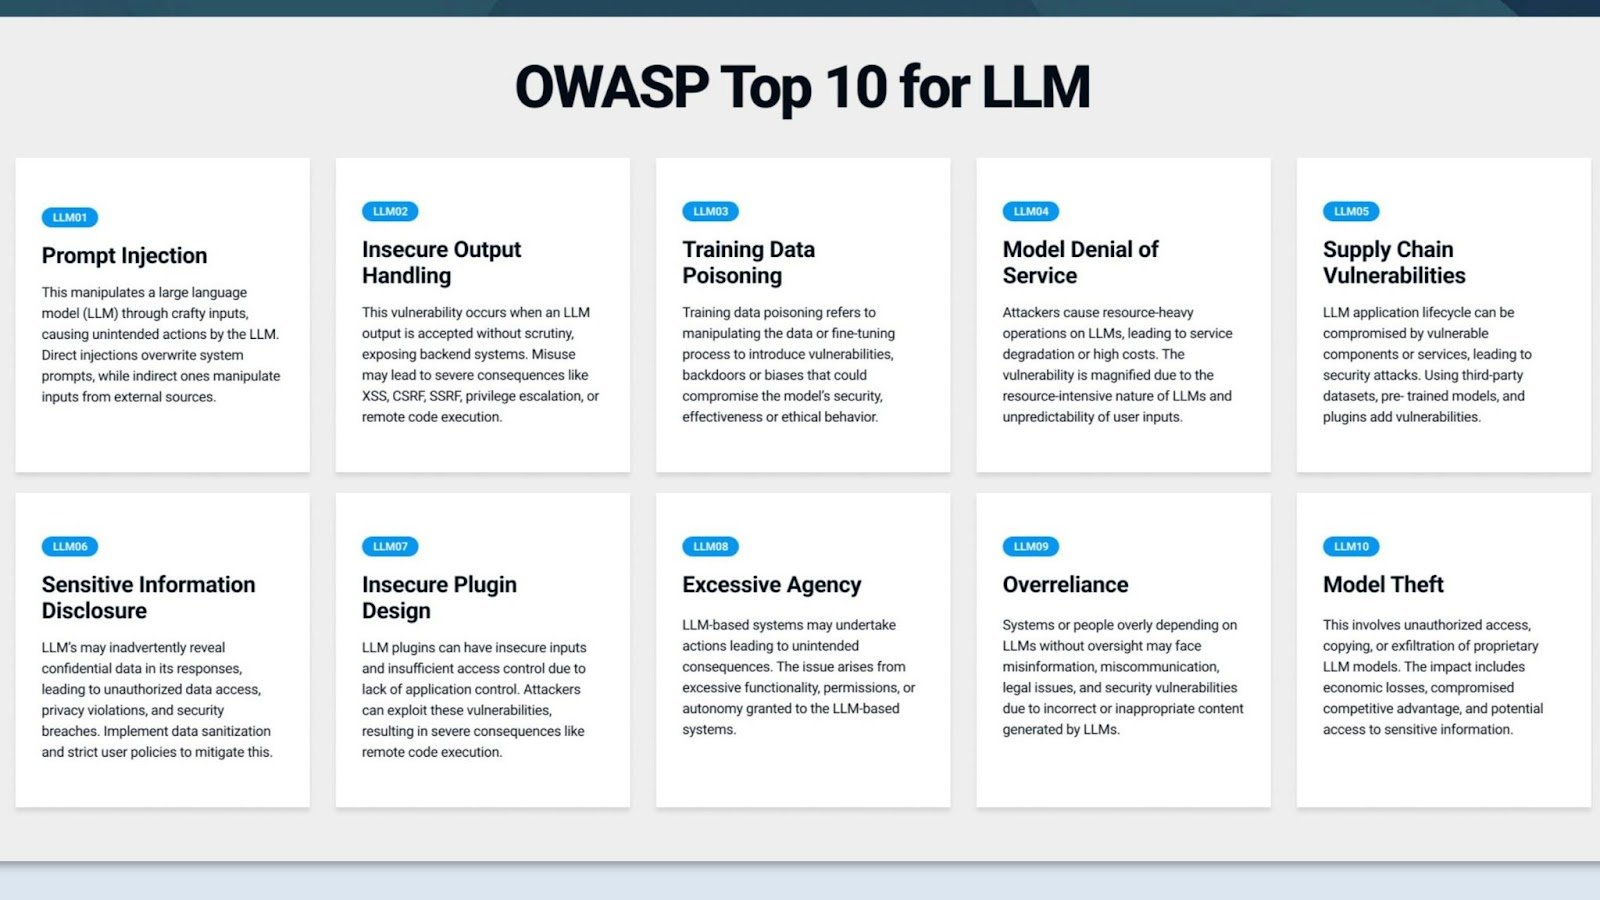
\includegraphics[width=0.8\textwidth]{owasp_top_10_llm_highlevel}
  \caption{Image of OWASP Top 10 for Large Language Model Applications}
  \label{fig:owasp-top-10-llm-highlevel}
\end{figure}

\clearpage
\textbf{OWASP Top 10 for Large Language Model Applications Visualized}
\begin{figure}[ht]
  \centering
  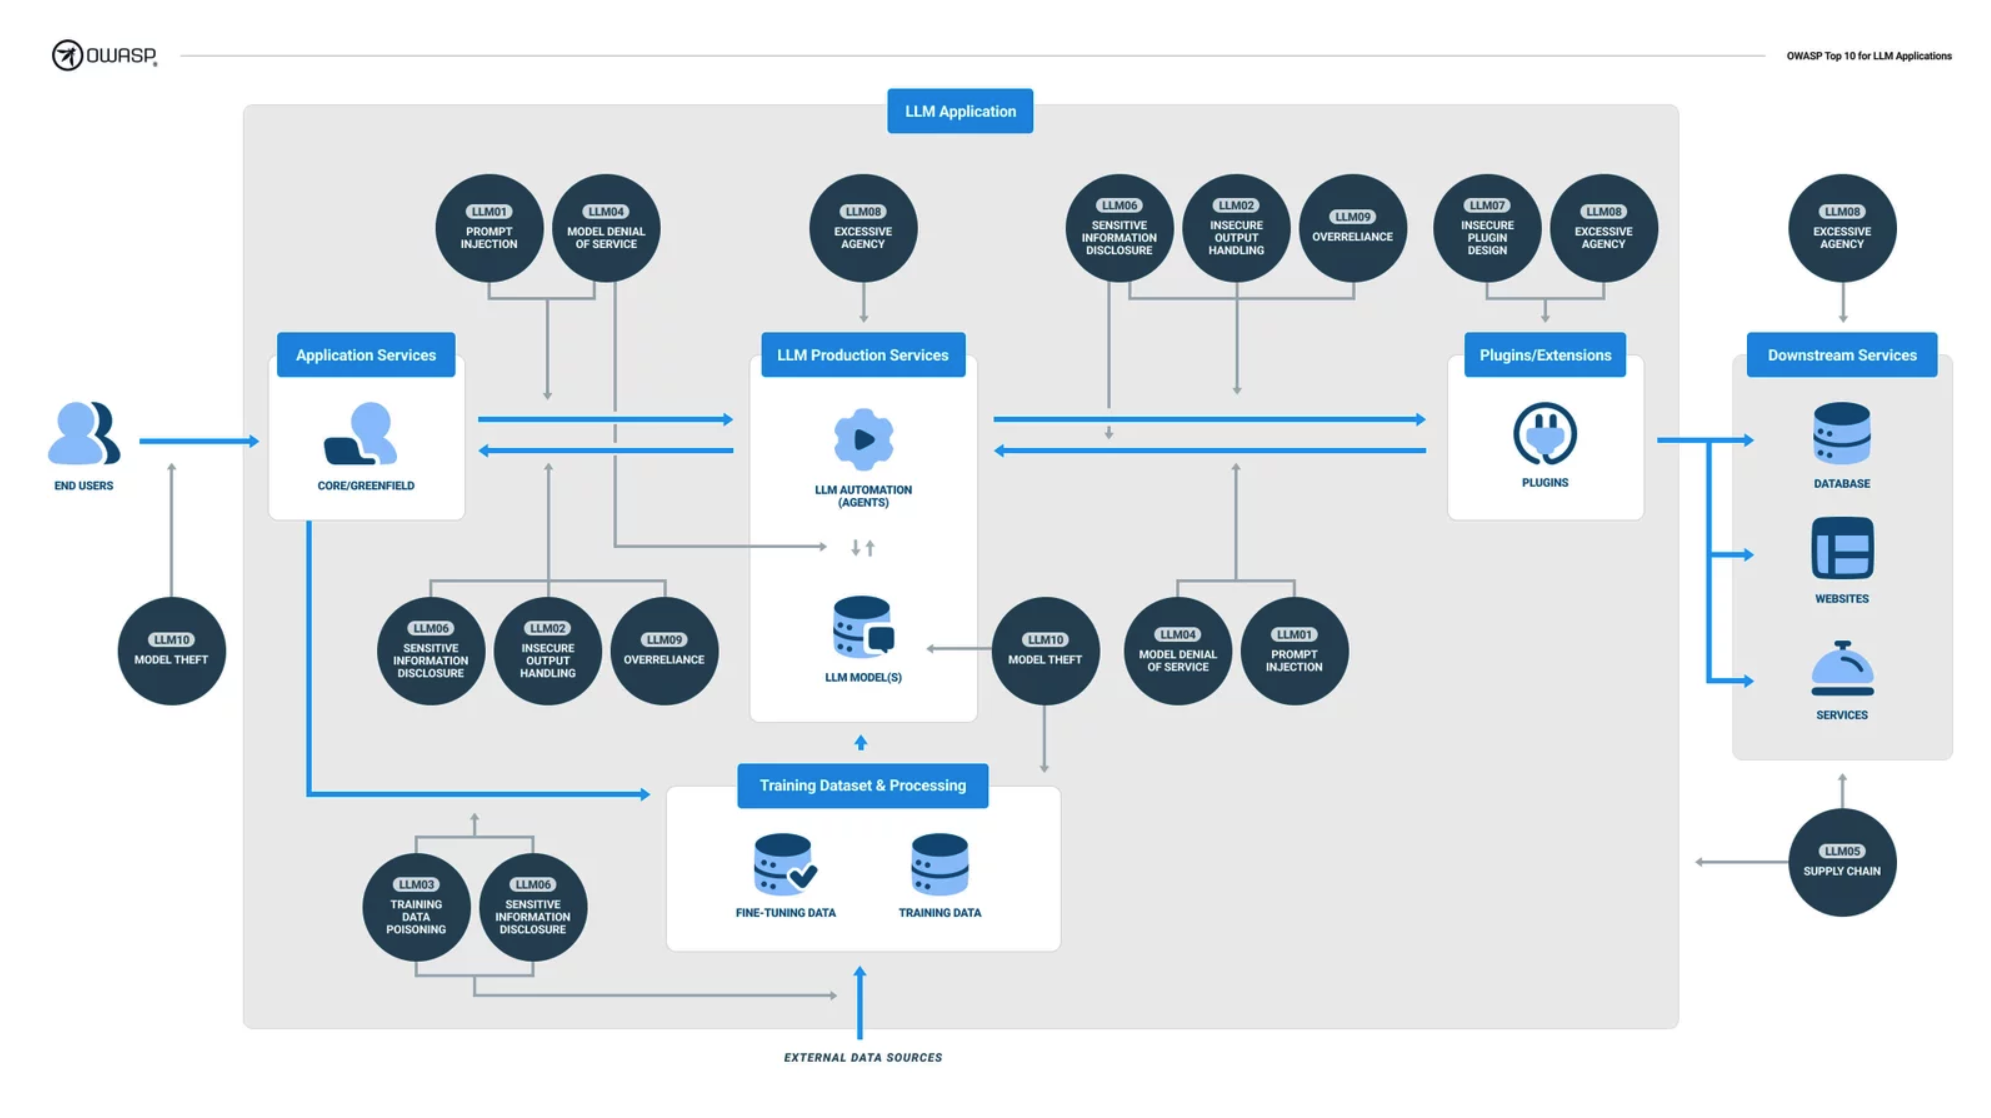
\includegraphics[width=0.8\textwidth]{owasp_top_10_llm_app_arch}
  \caption{Image of OWASP Top 10 for Large Language Model Applications Visualized}
  \label{fig:owasp-top-10-llm-visualized}
\end{figure}

\clearpage
\textbf{OWASP Resources}
Using LLM solutions expands an organization's attack surface and presents new
challenges, requiring special tactics and defenses. It also poses problems that
are similar to known issues, and there are already established cybersecurity
procedures and mitigations. Integrating LLM cybersecurity with an organization's
established cybersecurity controls, processes, and procedures allows an
organization to reduce its vulnerability to threats. How they integrate with
each other is available at the
\href{https://owasp.org/www-project-integration-standards/}{OWASP Integration Standards}.
%%% TABLE FORMATTING
\setlength\LTleft{0pt}
\setlength\LTright{0pt}
\begin{longtable}[c]{|p{0.25\textwidth}|p{0.25\textwidth}|p{0.35\textwidth}|}
  %%% Header and footer information
  \hline
  \rowcolor{owasplightpurple}
  \textbf{OWASP Resource} &
  \textbf{Description} &
  \textbf{Why It Is Recommended \& Where To Use It} \\
  \hline
  \endfirsthead
  \hline
  \rowcolor{owasplightpurple}
  \textbf{OWASP Resource} &
  \textbf{Description} &
  \textbf{Why It Is Recommended \& Where To Use It} \\
  \hline
  \endhead
  \endfoot
  %%% TABLE DATA GOES HERE
  \href{https://owasp.org/www-project-samm/}{OWASP SAMM}&
  Software Assurance Maturity Model &
  Provides an effective and measurable way to analyze and improve an
  organization's secure development lifecycle. SAMM supports the complete
  software lifecycle. It is interative and risk-driven, enabling organizations
  to identify and prioritize gaps in secure software development so resources
  for improving the process can be dedicated where efforts have the greatest
  improvement impact. \\
  \hline
  \href{https://owasp.org/www-project-ai-security-and-privacy-guide/}{OWASP AI Security and Privacy Guide} &
  OWASP Project with a goal of connecting worldwide for an exchange on AI
  security, fostering standards alignment, and driving collaboration. &
  The OWASP AI Security and Privacy Guide is a comprehensive list of the most
  important AI security and privacy considerations. It is meant to be a
  comprehensive resource for developers, security researchers, and security
  consultants to verify the security and privacy of AI systems. \\
  \hline
  \href{https://owasp.org/www-project-ai-security/}{OWASP AI Exchange} &
  OWASP AI Exchange is the intake method for the OWASP AI Security and Privacy Guide. &
  The AI Exchange is the primary intake method used by OWASP to drive the direction of
  the OWASP AI Security and Privacy Guide. \\
  \hline
  \href{https://mltop10.info/}{OWASP Machine Learning Security Top 10} &
  OWASP Machine Learning Security Top 10 security issues of machine learning systems. &
  The OWASP Machine Learning Security Top 10 is a community-driven effort to
  collect and present the most important security issues of machine learning
  systems in a format that is easy to understand by both a security expert and
  a data scientist. This project includes the ML Top 10 and is a live working
  document that provides clear and actionable insights on designing, creating,
  testing, and procuring secure and privacy-preserving AI systems. It is the
  best OWASP resource for AI global regulatory and privacy information.\\
  \hline
  \href{https://www.opencre.org/}{OpenCRE} &
  OpenCRE (Common Requirement Enumeration) is the interactive content-linking
  platform for uniting security standards and guidelines into one overview. &
  Use this site to search for standards. You can search by standard name or by
  control type.  \\
  \hline
  \href{https://owasp.org/www-community/Threat_Modeling}{OWASP Threat Modeling} &
  A structured, formal process for threat modeling of an application &
  Learn everything about Threat Modeling which is a structured representation
  of all the information that affects the security of an application. \\
  \hline
  \href{https://owasp.org/www-project-cyclonedx/}{OWASP CycloneDX} &
  OWASP CycloneDX is a full-stack Bill of Materials (BOM) standard that
  provides advanced supply chain capabilities for cyber risk reduction. &
  Modern software is assembled using third-party and open source components.
  They are glued together in complex and unique ways and integrated with
  original code to achieve the desired functionality. An SBOM provides an
  accurate inventory of all components which enables organizations to identify
  risk, allows for greater transparency, and enables rapid impact analysis.
  \href{https://www.nist.gov/itl/executive-order-14028-improving-nations-cybersecurity/software-security-supply-chains-software-1}{EO 14028}
  provided minimum requirements for SBOM for federal systems. \\
  \hline
  \href{https://scvs.owasp.org/}{OWASP Software Component Verification Standard (SCVS) } &
  A community-driven effort to establish a framework for identifying activities,
  controls, and best practices can help in identifying and reducing risk in a
  software supply chain. &
  Use SCVS to develop a common set of activities, controls, and best-practices
  that can reduce risk in a software supply chain and identify a baseline and
  path to mature software supply chain vigilance. \\
  \hline
  \href{https://owasp.org/www-project-api-security/}{OWASP API Security Project } &
  API Security focuses on strategies and solutions to understand and mitigate
  the unique vulnerabilities and security risks of Application Programming
  Interfaces (APIs) &
  APIs are a foundational element of connecting applications, and mitigating
  misconfigurations or vulnerabilities is mandatory to protect users and
  organizations. Use for security testing and red teaming the build and
  production environments. \\
  \hline
  \href{https://owasp.org/www-project-application-security-verification-standard/}{OWASP Application Security Verification Standard ASVS} &
  Application Security Verification Standard (ASVS) Project provides a basis
  for testing web application technical security controls and also provides
  developers with a list of requirements for secure development. &
  Cookbook for web application security requirements, security testing, and
  metrics. Use to establish security user stories and security use case release
  testing. \\
  \hline
  \href{https://owasp.org/www-project-threat-and-safeguard-matrix/}{OWASP Threat and Safeguard Matrix (TaSM)} &
  An action oriented view to safeguard and enable the business &
  This matrix allows a company to overlay its major threats with the NIST Cyber
  Security Framework Functions (Identify, Protect, Detect, Respond, \& Recover)
  to build a robust security plan. Use it as a dashboard to track and report on
  security across the organization. \\
  \hline
  \href{https://www.defectdojo.com/}{Defect Dojo} &
  An open source vulnerability management tool that streamlines the testing
  process by offering templating, report generation, metrics, and baseline
  self-service tools. &
  Use Defect Dojo to reduce the time for logging vulnerabilities with templates
  for vulnerabilities, imports for common vulnerability scanners, report
  generation, and metrics. \\
  \hline
  %%% TABLE DATA ENDS HERE
  \caption{OWASP Resources}
  \label{tab:owasp-resources}
\end{longtable}

% !TEX root = owasp-doc.tex
\clearpage
\textbf{MITRE Resources}
The increased frequency of LLM threats emphasizes the value of a
resilience-first approach to defending an organization's attack surface.
Existing TTPS are combined with new attack surfaces and capabilities in LLM
Adversary threats and mitigations. MITRE maintains a well-established and
widely accepted mechanism for coordinating opponent tactics and procedures
based on real-world observations.

Coordination and mapping of an organization's LLM Security Strategy to MITRE
ATT\&CK and MITRE ATLAS allows an organization to determine where LLM Security
is covered by current processes such as API Security Standards or where
security holes exists.

MITRE ATT\&CK (Adversarial Tactics, Techniques, and Common Knowledge) is a
framework, collection of data matrices, and assessment tool that was made by
the MITRE Corporation to help organizations figure out how well their
cybersecurity works across their entire digital attack surface and find holes
that had not been found before. It is a knowledge repository that is used all
over the world. The MITRE ATT\&CK matrix contains a collection of strategies
used by adversaries to achieve a certain goal. In the ATT\&CK Matrix, these
objectives are classified as tactics. The objectives are outlined in attack
order, beginning with reconnaissance and progressing to the eventual goal of
exfiltration or impact.

MITRE ATLAS, which stands for "Adversarial Threat Landscape for Artificial
Intelligence Systems," is a knowledge base that is based on real-life examples
of attacks on machine learning (ML) systems by bad actors. ATLAS is based on the
MITRE ATT\&CK architecture, and its tactics and procedures complement those
found in ATT\&CK.
%%% TABLE FORMATTING
\setlength\LTleft{0pt}
\setlength\LTright{0pt}
\begin{longtable}[c]{|p{0.25\textwidth}|p{0.25\textwidth}|p{0.35\textwidth}|}
  %%% Header and footer information
  \hline
  \rowcolor{owasplightpurple}
  \textbf{MITRE Resource} &
  \textbf{Description} &
  \textbf{Why It Is Recommended \& Where To Use It} \\
  \hline
  \endfirsthead
  \hline
  \rowcolor{owasplightpurple}
  \textbf{MITRE Resource} &
  \textbf{Description} &
  \textbf{Why It Is Recommended \& Where To Use It} \\
  \hline
  \endhead
  \endfoot
  %%% TABLE DATA STARTS HERE
  \href{https://attack.mitre.org/}{MITRE ATT\&CK} &
  Knowledge base of adversary tactics and techniques based on real-world observations &
  The ATT\&CK knowledge base is used as a foundation for the development of
  specific threat models and methodologies. Map existing controls within the
  organization to adversary tactics and techniques to identify gaps or areas to
  test. \\
  \hline
  \href{https://medium.com/mitre-engenuity/att-ck-workbench-2-0-your-bench-your-team-your-most-relevant-ttps-5b9620457ef4}{MITRE AT\&CK Workbench} &
  Create or extend ATT\&CK data in a local knowledge base &
  Host and manage a customized copy of the ATT\&CK knowledge base. This local
  copy of the ATT\&CK knowledge base can be extended with new or updated
  techniques, tactics, mitigation groups, and software that is specific to your
  organization. \\
  \hline
  \href{https://atlas.mitre.org/}{MITRE ATLAS} &
  MITRE ATLAS (Adversarial Threat Landscape for Artificial-Intelligence Systems)
  is a knowledge base of adversary tactics, techniques, and case studies for
  machine learning (ML) systems based on real-world observations, demonstrations
  from ML red teams and security groups, and the state of the possible from
  academic research &
  Use it to map known ML vulnerabilities and map checks and controls for
  proposed projects or existing systems. \\
  \hline
  \href{https://mitre-engenuity.org/cybersecurity/center-for-threat-informed-defense/attack-powered-suit/}{MITRE ATT\&CK Powered Suit} &
  ATT\&CK Powered Suit is a browser extension that puts the MITRE ATT\&CK
  knowledge base at your fingertips. &
  Add to your browser to quickly search for tactics, techniques, and more
  without disrupting your workflow. \\
  \hline
  \href{https://mitre-engenuity.org/cybersecurity/center-for-threat-informed-defense/our-work/threat-report-attck-mapper-tram/}{The Threat Report ATT\&CK Mapper (TRAM)} &
  Automates TTP Identification in CTI Reports &
  Mapping TTPs found in CTI reports to MITRE ATT\&CK is difficult, error prone,
  and time-consuming. TRAM uses LLMs to automate this process for the 50 most
  common techniques. Supports Juypter notebooks. \\
  \hline
  \href{https://center-for-threat-informed-defense.github.io/attack-flow/}{Attack Flow v2.1.0} &
  Attack Flow is a language for describing how cyber adversaries combine and
  sequence various offensive techniques to achieve their goals.  &
  Attack Flow helps visualize how an attacker uses a technique, so defenders
  and leaders understand how adversaries operate and improve their own
  defensive posture. \\
  \hline
  \href{https://caldera.mitre.org/}{MITRE Caldera} &
  A cyber security platform (framework) designed to easily automate adversary
  emulation, assist manual red-teams, and automate incident response. &
  \href{https://caldera.readthedocs.io/en/latest/Plugin-library.html}{Plugins} are available for Caldera that help to expand the core capabilities
  of the framework and provide additional functionality, including agents,
  reporting, collections of TTPs and others
 \\
  \hline
  \href{https://github.com/mitre-atlas/arsenal}{CALDERA plugin: Arsenal} &
  A plugin developed for adversary emulation of AI-enabled systems.  &
  This plugin provides TTPs defined in MITRE ATLAS to interface with CALDERA. \\
  \hline
  \href{https://github.com/redcanaryco/atomic-red-team}{Atomic Red Team} &
  Library of tests mapped to the MITRE ATT\&CK framework. &
  Use to validate and test controls in an environment. Security teams can use
  Atomic Red Team to quickly, portably, and reproducibly test their environments.
  You can execute atomic tests directly from the command line; no installation
  is required.
 \\
  \hline
  \href{https://mitre-engenuity.org/cybersecurity/center-for-threat-informed-defense/our-work/cti-blueprints/}{MITRE CTI Blueprints} &
  Automates Cyber Threat Intelligence reporting. &
  CTI Blueprints helps Cyber Threat Intelligence (CTI) analysts create
  high-quality, actionable reports more consistently and efficiently.
 \\
  \hline
  %%% TABLE DATA ENDS HERE
  \caption{MITRE Resources}
  \label{tab:mitre-resources}
\end{longtable}
% !TEX root = owasp-doc.tex

\clearpage
\section{AI Vulnerability Repositories}

%%% TABLE FORMATTING
\setlength\LTleft{0pt}
\setlength\LTright{0pt}
\begin{longtable}[c]{|p{0.45\textwidth}|p{0.55\textwidth}|}
  %%% Header and footer information
  \hline
  \rowcolor{owasplightpurple}
  \textbf{Name} &
  \textbf{Description}\\
  \hline
  \endfirsthead
  \hline
  \rowcolor{owasplightpurple}
  \textbf{Name} &
  \textbf{Description} \\
  \hline
  \endhead
  \endfoot
  %%% TABLE DATA STARTS HERE
  \href{https://incidentdatabase.ai/}{AI Incident Database} &
  A repository of articles about different times AI has failed in real-world
  applications and is maintained by a college research group and crowds sourced. \\
  \hline
  \href{https://oecd.ai/en/incidents}{OECD AI Incidents Monitor (AIM)} &
  Offers an accessible starting point for comprehending the landscape of AI-related challenges. \\
  \hline
  \rowcolor{owasplightpurple}
  \multicolumn{2}{|c|}{
    \textbf{Three of the leading companies tracking AI Model vulnerabilities}
  } \\
  \hline
  \href{https://huntr.com/}{Huntr Bug Bounty : ProtectAI} &
  Bug bounty platform for AI/ML \\
  \hline
  \href{https://avidml.gitbook.io/}{AI Vulnerability Database (AVID) : \href{https://garak.ai/}{Garak}} &
  Database of model vulnerabilities  \\
  \hline
  \href{https://airisk.io/}{AI Risk Database: Robust Intelligence} &
  Database of model vulnerabilities  \\
  \hline
  %%% TABLE DATA ENDS HERE
  \caption{AI Vulnerability Repositories}
  \label{tab:ai-vulnerability-repositories}
\end{longtable}

% !TEX root = owasp-doc.tex
\clearpage
\textbf{AI Procurement Guidance}
%%% TABLE FORMATTING
\setlength\LTleft{0pt}
\setlength\LTright{0pt}
\begin{longtable}[c]{|p{0.45\textwidth}|p{0.55\textwidth}|}
  %%% Header and footer information
  \hline
  \rowcolor{owasplightpurple}
  \textbf{Name} &
  \textbf{Description} \\
  \hline
  \endfirsthead
  \hline
  \rowcolor{owasplightpurple}
  \textbf{Name} &
  \textbf{Description} \\
  \hline
  \endhead
  \endfoot
  %%% TABLE DATA STARTS HERE
  \href{https://www3.weforum.org/docs/WEF_Adopting_AI_Responsibly_Guidelines_for_Procurement_of_AI_Solutions_by_the_Private_Sector_2023.pdf}{World Economic Forum: Adopting AI Responsibly: Guidelines for Procurement of AI Solutions by the Private Sector: Insight Report June 2023} &
  The standard benchmarks and assessment criteria for procuring Artificial
  systems are in early development. The procurement guidelines provide
  organizations with a baseline of considerations for the end-to-end
  procurement process.

  Use this guidance to augment an organization's existing Third Party Risk
  Supplier and Vendor procurement process. \\
  \hline
  %%% TABLE DATA ENDS HERE
  \caption{AI Procurement Guidance}
  \label{tab:ai-procurement-guidance}
\end{longtable}
\clearpage

%%% APPENDICES
\appendix
% !TEX root = report.tex

% ------------------------------------------------
% TEAM
% ------------------------------------------------

\headerimage
\chapter{Team}

Thank you to the OWASP Top 10 for LLM Applications Cybersecurity and Governance
Checklist Contributors.

%%% TABLE FORMATTING
\setlength\LTleft{0pt}
\setlength\LTright{0pt}
\begin{longtable}[c]{|p{0.33\textwidth}|p{0.33\textwidth}|p{0.33\textwidth}|}
  %%% Header and footer information
  \hline
  \rowcolor{owasplightpurple}
  \multicolumn{3}{|c|}{
    \textbf{Checklist Contributors}
  } \\
  \hline
  \endfirsthead
  \hline
  \multicolumn{3}{|c|}{
    \textbf{Checklist Contributors}
  } \\
  \hline
  \endhead
  \endfoot
  %%% TABLE DATA GOES HERE
\hline
  Sandy Dunn & Heather Linn & \href{mailto:john.sotiropoulos@kainos.com}{John Sotiropoulos}   \\
  \hline
  Steve Wilson & Fabrizio Cilli & Aubrey King     \\
  \hline
  Bob Simonoff & David Rowe & \href{mailto:r.vanderveer@sig.eu}{Rob Vanderveer}      \\
  \hline
  Emmanual Guilherme Junior & Andrea Succi & Jason Ross \\
  \hline
  Talesh Seeparsan & Anthony Glynn & Julie Tao \\
  \hline
  %%% TABLE DATA ENDS HERE
  \caption{OWASP LLM AI Security \& Governance Checklist Team}
  \label{tab:team}
\end{longtable}

This project is licensed under the terms of the
\href{https://creativecommons.org/licenses/by-sa/4.0/}{Creative Commons Attribution-ShareAlike 4.0 International License}

\end{document}
% \tracingmacros=0 % turn off tracing